\section{Order of events}

\code{model/scheduler.py} runs one period; each step sees only what earlier steps produced.

\begin{enumerate}
\item \textbf{Start.} Plants bought last period arrive; flows are reset.
\item \textbf{Pricing.} Firms post $p_i$ from last period's prices, utilisation and leader.
\item \textbf{Demand.} Shares from prices, demand allocated within capacity, sales and utilisation.
\item \textbf{Production and accounts.} Plants run in merit order; profits, dividends, cash and debt.
\item \textbf{Scrapping.} Hurdles are updated; plants retire by age or obsolescence; replacement.
\item \textbf{Investment.} Desired capacity, technique chosen with $h$, finance; plants arrive next period.
\item \textbf{Entry and exit,} then the collector and the stock-flow check.
\end{enumerate}

\begin{figure}[h]
\centering
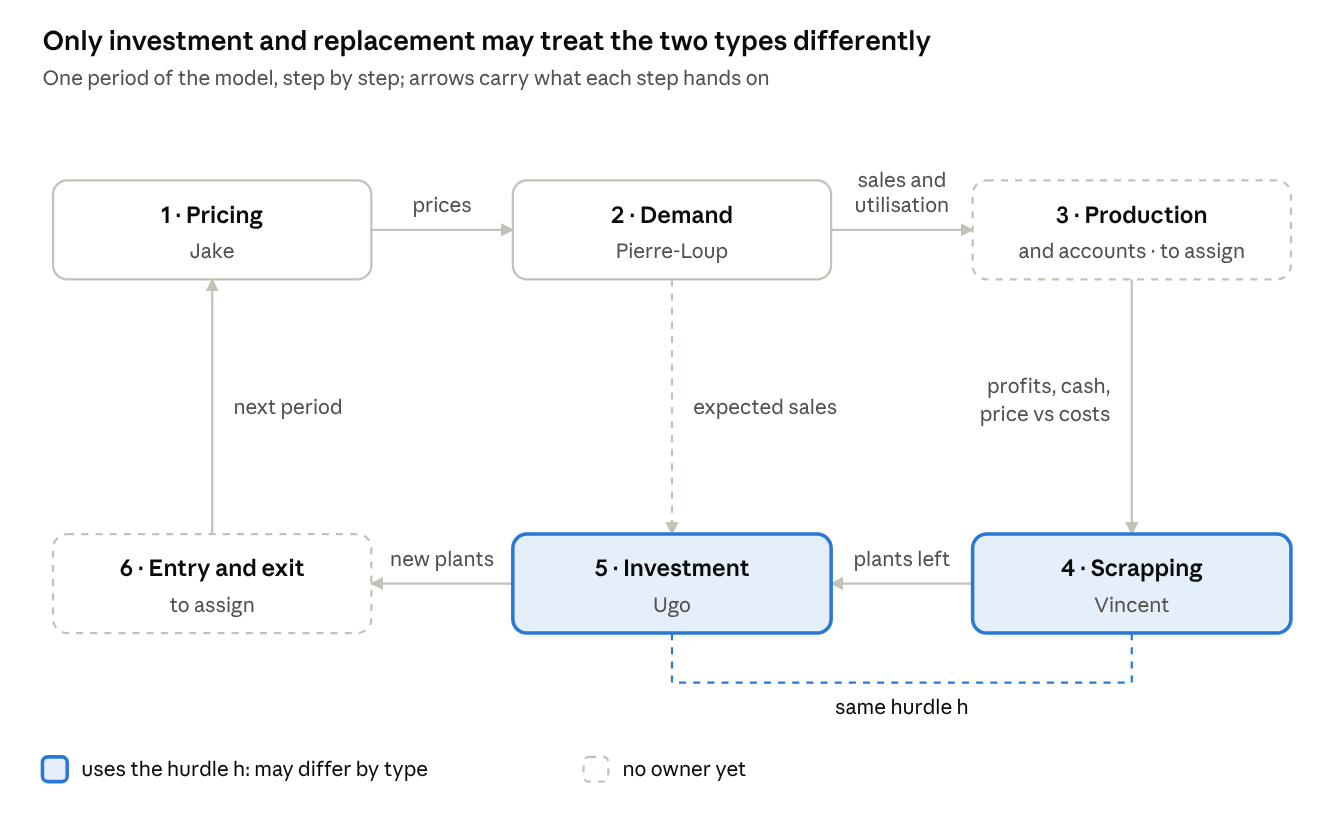
\includegraphics[width=0.7\textwidth]{../docs/design/img/2026-10-16_ABM-Project_mechanism-briefs_one-period.png}
\caption{One period: six steps, one shared hurdle (from the briefs).}
\end{figure}

\schedulerpart{period}{\code{model/scheduler.py}: one period}
